%% template.tex
%% from
%% bare_conf.tex
%% V1.4b
%% 2015/08/26
%% by Michael Shell
%% See:
%% http://www.michaelshell.org/
%% for current contact information.
%%
%% This is a skeleton file demonstrating the use of IEEEtran.cls
%% (requires IEEEtran.cls version 1.8b or later) with an IEEE
%% conference paper.
%%
%% Support sites:
%% http://www.michaelshell.org/tex/ieeetran/
%% http://www.ctan.org/pkg/ieeetran
%% and
%% http://www.ieee.org/

%%*************************************************************************
%% Legal Notice:
%% This code is offered as-is without any warranty either expressed or
%% implied; without even the implied warranty of MERCHANTABILITY or
%% FITNESS FOR A PARTICULAR PURPOSE!
%% User assumes all risk.
%% In no event shall the IEEE or any contributor to this code be liable for
%% any damages or losses, including, but not limited to, incidental,
%% consequential, or any other damages, resulting from the use or misuse
%% of any information contained here.
%%
%% All comments are the opinions of their respective authors and are not
%% necessarily endorsed by the IEEE.
%%
%% This work is distributed under the LaTeX Project Public License (LPPL)
%% ( http://www.latex-project.org/ ) version 1.3, and may be freely used,
%% distributed and modified. A copy of the LPPL, version 1.3, is included
%% in the base LaTeX documentation of all distributions of LaTeX released
%% 2003/12/01 or later.
%% Retain all contribution notices and credits.
%% ** Modified files should be clearly indicated as such, including  **
%% ** renaming them and changing author support contact information. **
%%*************************************************************************


% *** Authors should verify (and, if needed, correct) their LaTeX system  ***
% *** with the testflow diagnostic prior to trusting their LaTeX platform ***
% *** with production work. The IEEE's font choices and paper sizes can   ***
% *** trigger bugs that do not appear when using other class files.       ***                          ***
% The testflow support page is at:
% http://www.michaelshell.org/tex/testflow/

\documentclass[conference,final,]{IEEEtran}
% Some Computer Society conferences also require the compsoc mode option,
% but others use the standard conference format.
%
% If IEEEtran.cls has not been installed into the LaTeX system files,
% manually specify the path to it like:
% \documentclass[conference]{../sty/IEEEtran}





% Some very useful LaTeX packages include:
% (uncomment the ones you want to load)


% *** MISC UTILITY PACKAGES ***
%
%\usepackage{ifpdf}
% Heiko Oberdiek's ifpdf.sty is very useful if you need conditional
% compilation based on whether the output is pdf or dvi.
% usage:
% \ifpdf
%   % pdf code
% \else
%   % dvi code
% \fi
% The latest version of ifpdf.sty can be obtained from:
% http://www.ctan.org/pkg/ifpdf
% Also, note that IEEEtran.cls V1.7 and later provides a builtin
% \ifCLASSINFOpdf conditional that works the same way.
% When switching from latex to pdflatex and vice-versa, the compiler may
% have to be run twice to clear warning/error messages.






% *** CITATION PACKAGES ***
%
%\usepackage{cite}
% cite.sty was written by Donald Arseneau
% V1.6 and later of IEEEtran pre-defines the format of the cite.sty package
% \cite{} output to follow that of the IEEE. Loading the cite package will
% result in citation numbers being automatically sorted and properly
% "compressed/ranged". e.g., [1], [9], [2], [7], [5], [6] without using
% cite.sty will become [1], [2], [5]--[7], [9] using cite.sty. cite.sty's
% \cite will automatically add leading space, if needed. Use cite.sty's
% noadjust option (cite.sty V3.8 and later) if you want to turn this off
% such as if a citation ever needs to be enclosed in parenthesis.
% cite.sty is already installed on most LaTeX systems. Be sure and use
% version 5.0 (2009-03-20) and later if using hyperref.sty.
% The latest version can be obtained at:
% http://www.ctan.org/pkg/cite
% The documentation is contained in the cite.sty file itself.






% *** GRAPHICS RELATED PACKAGES ***
%
\ifCLASSINFOpdf
  % \usepackage[pdftex]{graphicx}
  % declare the path(s) where your graphic files are
  % \graphicspath{{../pdf/}{../jpeg/}}
  % and their extensions so you won't have to specify these with
  % every instance of \includegraphics
  % \DeclareGraphicsExtensions{.pdf,.jpeg,.png}
\else
  % or other class option (dvipsone, dvipdf, if not using dvips). graphicx
  % will default to the driver specified in the system graphics.cfg if no
  % driver is specified.
  % \usepackage[dvips]{graphicx}
  % declare the path(s) where your graphic files are
  % \graphicspath{{../eps/}}
  % and their extensions so you won't have to specify these with
  % every instance of \includegraphics
  % \DeclareGraphicsExtensions{.eps}
\fi
% graphicx was written by David Carlisle and Sebastian Rahtz. It is
% required if you want graphics, photos, etc. graphicx.sty is already
% installed on most LaTeX systems. The latest version and documentation
% can be obtained at:
% http://www.ctan.org/pkg/graphicx
% Another good source of documentation is "Using Imported Graphics in
% LaTeX2e" by Keith Reckdahl which can be found at:
% http://www.ctan.org/pkg/epslatex
%
% latex, and pdflatex in dvi mode, support graphics in encapsulated
% postscript (.eps) format. pdflatex in pdf mode supports graphics
% in .pdf, .jpeg, .png and .mps (metapost) formats. Users should ensure
% that all non-photo figures use a vector format (.eps, .pdf, .mps) and
% not a bitmapped formats (.jpeg, .png). The IEEE frowns on bitmapped formats
% which can result in "jaggedy"/blurry rendering of lines and letters as
% well as large increases in file sizes.
%
% You can find documentation about the pdfTeX application at:
% http://www.tug.org/applications/pdftex





% *** MATH PACKAGES ***
%
%\usepackage{amsmath}
% A popular package from the American Mathematical Society that provides
% many useful and powerful commands for dealing with mathematics.
%
% Note that the amsmath package sets \interdisplaylinepenalty to 10000
% thus preventing page breaks from occurring within multiline equations. Use:
%\interdisplaylinepenalty=2500
% after loading amsmath to restore such page breaks as IEEEtran.cls normally
% does. amsmath.sty is already installed on most LaTeX systems. The latest
% version and documentation can be obtained at:
% http://www.ctan.org/pkg/amsmath





% *** SPECIALIZED LIST PACKAGES ***
%
%\usepackage{algorithmic}
% algorithmic.sty was written by Peter Williams and Rogerio Brito.
% This package provides an algorithmic environment fo describing algorithms.
% You can use the algorithmic environment in-text or within a figure
% environment to provide for a floating algorithm. Do NOT use the algorithm
% floating environment provided by algorithm.sty (by the same authors) or
% algorithm2e.sty (by Christophe Fiorio) as the IEEE does not use dedicated
% algorithm float types and packages that provide these will not provide
% correct IEEE style captions. The latest version and documentation of
% algorithmic.sty can be obtained at:
% http://www.ctan.org/pkg/algorithms
% Also of interest may be the (relatively newer and more customizable)
% algorithmicx.sty package by Szasz Janos:
% http://www.ctan.org/pkg/algorithmicx




% *** ALIGNMENT PACKAGES ***
%
%\usepackage{array}
% Frank Mittelbach's and David Carlisle's array.sty patches and improves
% the standard LaTeX2e array and tabular environments to provide better
% appearance and additional user controls. As the default LaTeX2e table
% generation code is lacking to the point of almost being broken with
% respect to the quality of the end results, all users are strongly
% advised to use an enhanced (at the very least that provided by array.sty)
% set of table tools. array.sty is already installed on most systems. The
% latest version and documentation can be obtained at:
% http://www.ctan.org/pkg/array


% IEEEtran contains the IEEEeqnarray family of commands that can be used to
% generate multiline equations as well as matrices, tables, etc., of high
% quality.




% *** SUBFIGURE PACKAGES ***
%\ifCLASSOPTIONcompsoc
%  \usepackage[caption=false,font=normalsize,labelfont=sf,textfont=sf]{subfig}
%\else
%  \usepackage[caption=false,font=footnotesize]{subfig}
%\fi
% subfig.sty, written by Steven Douglas Cochran, is the modern replacement
% for subfigure.sty, the latter of which is no longer maintained and is
% incompatible with some LaTeX packages including fixltx2e. However,
% subfig.sty requires and automatically loads Axel Sommerfeldt's caption.sty
% which will override IEEEtran.cls' handling of captions and this will result
% in non-IEEE style figure/table captions. To prevent this problem, be sure
% and invoke subfig.sty's "caption=false" package option (available since
% subfig.sty version 1.3, 2005/06/28) as this is will preserve IEEEtran.cls
% handling of captions.
% Note that the Computer Society format requires a larger sans serif font
% than the serif footnote size font used in traditional IEEE formatting
% and thus the need to invoke different subfig.sty package options depending
% on whether compsoc mode has been enabled.
%
% The latest version and documentation of subfig.sty can be obtained at:
% http://www.ctan.org/pkg/subfig




% *** FLOAT PACKAGES ***
%

%\usepackage{fixltx2e}
% fixltx2e, the successor to the earlier fix2col.sty, was written by
% Frank Mittelbach and David Carlisle. This package corrects a few problems
% in the LaTeX2e kernel, the most notable of which is that in current
% LaTeX2e releases, the ordering of single and double column floats is not
% guaranteed to be preserved. Thus, an unpatched LaTeX2e can allow a
% single column figure to be placed prior to an earlier double column
% figure.
% Be aware that LaTeX2e kernels dated 2015 and later have fixltx2e.sty's
% corrections already built into the system in which case a warning will
% be issued if an attempt is made to load fixltx2e.sty as it is no longer
% needed.
% The latest version and documentation can be found at:
% http://www.ctan.org/pkg/fixltx2e


%\usepackage{stfloats}
% stfloats.sty was written by Sigitas Tolusis. This package gives LaTeX2e
% the ability to do double column floats at the bottom of the page as well
% as the top. (e.g., "\begin{figure*}[!b]" is not normally possible in
% LaTeX2e). It also provides a command:
%\fnbelowfloat
% to enable the placement of footnotes below bottom floats (the standard
% LaTeX2e kernel puts them above bottom floats). This is an invasive package
% which rewrites many portions of the LaTeX2e float routines. It may not work
% with other packages that modify the LaTeX2e float routines. The latest
% version and documentation can be obtained at:
% http://www.ctan.org/pkg/stfloats
% Do not use the stfloats baselinefloat ability as the IEEE does not allow
% \baselineskip to stretch. Authors submitting work to the IEEE should note
% that the IEEE rarely uses double column equations and that authors should try
% to avoid such use. Do not be tempted to use the cuted.sty or midfloat.sty
% packages (also by Sigitas Tolusis) as the IEEE does not format its papers in
% such ways.
% Do not attempt to use stfloats with fixltx2e as they are incompatible.
% Instead, use Morten Hogholm'a dblfloatfix which combines the features
% of both fixltx2e and stfloats:
%
% \usepackage{dblfloatfix}
% The latest version can be found at:
% http://www.ctan.org/pkg/dblfloatfix




% *** PDF, URL AND HYPERLINK PACKAGES ***
%
%\usepackage{url}
% url.sty was written by Donald Arseneau. It provides better support for
% handling and breaking URLs. url.sty is already installed on most LaTeX
% systems. The latest version and documentation can be obtained at:
% http://www.ctan.org/pkg/url
% Basically, \url{my_url_here}.




% *** Do not adjust lengths that control margins, column widths, etc. ***
% *** Do not use packages that alter fonts (such as pslatex).         ***
% There should be no need to do such things with IEEEtran.cls V1.6 and later.
% (Unless specifically asked to do so by the journal or conference you plan
% to submit to, of course. )



%% BEGIN MY ADDITIONS %%


\usepackage{graphicx}
% We will generate all images so they have a width \maxwidth. This means
% that they will get their normal width if they fit onto the page, but
% are scaled down if they would overflow the margins.
\makeatletter
\def\maxwidth{\ifdim\Gin@nat@width>\linewidth\linewidth
\else\Gin@nat@width\fi}
\makeatother
\let\Oldincludegraphics\includegraphics
\renewcommand{\includegraphics}[1]{\Oldincludegraphics[width=\maxwidth]{#1}}

\usepackage[unicode=true]{hyperref}

\hypersetup{
            pdftitle={Predicting Fire Behavior Using Weather \& Meteorological Data},
            pdfborder={0 0 0},
            breaklinks=true}
\urlstyle{same}  % don't use monospace font for urls

% Pandoc toggle for numbering sections (defaults to be off)
\setcounter{secnumdepth}{0}

% Pandoc syntax highlighting
\usepackage{color}
\usepackage{fancyvrb}
\newcommand{\VerbBar}{|}
\newcommand{\VERB}{\Verb[commandchars=\\\{\}]}
\DefineVerbatimEnvironment{Highlighting}{Verbatim}{commandchars=\\\{\}}
% Add ',fontsize=\small' for more characters per line
\usepackage{framed}
\definecolor{shadecolor}{RGB}{248,248,248}
\newenvironment{Shaded}{\begin{snugshade}}{\end{snugshade}}
\newcommand{\AlertTok}[1]{\textcolor[rgb]{0.94,0.16,0.16}{#1}}
\newcommand{\AnnotationTok}[1]{\textcolor[rgb]{0.56,0.35,0.01}{\textbf{\textit{#1}}}}
\newcommand{\AttributeTok}[1]{\textcolor[rgb]{0.77,0.63,0.00}{#1}}
\newcommand{\BaseNTok}[1]{\textcolor[rgb]{0.00,0.00,0.81}{#1}}
\newcommand{\BuiltInTok}[1]{#1}
\newcommand{\CharTok}[1]{\textcolor[rgb]{0.31,0.60,0.02}{#1}}
\newcommand{\CommentTok}[1]{\textcolor[rgb]{0.56,0.35,0.01}{\textit{#1}}}
\newcommand{\CommentVarTok}[1]{\textcolor[rgb]{0.56,0.35,0.01}{\textbf{\textit{#1}}}}
\newcommand{\ConstantTok}[1]{\textcolor[rgb]{0.00,0.00,0.00}{#1}}
\newcommand{\ControlFlowTok}[1]{\textcolor[rgb]{0.13,0.29,0.53}{\textbf{#1}}}
\newcommand{\DataTypeTok}[1]{\textcolor[rgb]{0.13,0.29,0.53}{#1}}
\newcommand{\DecValTok}[1]{\textcolor[rgb]{0.00,0.00,0.81}{#1}}
\newcommand{\DocumentationTok}[1]{\textcolor[rgb]{0.56,0.35,0.01}{\textbf{\textit{#1}}}}
\newcommand{\ErrorTok}[1]{\textcolor[rgb]{0.64,0.00,0.00}{\textbf{#1}}}
\newcommand{\ExtensionTok}[1]{#1}
\newcommand{\FloatTok}[1]{\textcolor[rgb]{0.00,0.00,0.81}{#1}}
\newcommand{\FunctionTok}[1]{\textcolor[rgb]{0.00,0.00,0.00}{#1}}
\newcommand{\ImportTok}[1]{#1}
\newcommand{\InformationTok}[1]{\textcolor[rgb]{0.56,0.35,0.01}{\textbf{\textit{#1}}}}
\newcommand{\KeywordTok}[1]{\textcolor[rgb]{0.13,0.29,0.53}{\textbf{#1}}}
\newcommand{\NormalTok}[1]{#1}
\newcommand{\OperatorTok}[1]{\textcolor[rgb]{0.81,0.36,0.00}{\textbf{#1}}}
\newcommand{\OtherTok}[1]{\textcolor[rgb]{0.56,0.35,0.01}{#1}}
\newcommand{\PreprocessorTok}[1]{\textcolor[rgb]{0.56,0.35,0.01}{\textit{#1}}}
\newcommand{\RegionMarkerTok}[1]{#1}
\newcommand{\SpecialCharTok}[1]{\textcolor[rgb]{0.00,0.00,0.00}{#1}}
\newcommand{\SpecialStringTok}[1]{\textcolor[rgb]{0.31,0.60,0.02}{#1}}
\newcommand{\StringTok}[1]{\textcolor[rgb]{0.31,0.60,0.02}{#1}}
\newcommand{\VariableTok}[1]{\textcolor[rgb]{0.00,0.00,0.00}{#1}}
\newcommand{\VerbatimStringTok}[1]{\textcolor[rgb]{0.31,0.60,0.02}{#1}}
\newcommand{\WarningTok}[1]{\textcolor[rgb]{0.56,0.35,0.01}{\textbf{\textit{#1}}}}

% Pandoc header

\providecommand{\tightlist}{%
  \setlength{\itemsep}{0pt}\setlength{\parskip}{0pt}}

%% END MY ADDITIONS %%


\hyphenation{op-tical net-works semi-conduc-tor}

\begin{document}
%
% paper title
% Titles are generally capitalized except for words such as a, an, and, as,
% at, but, by, for, in, nor, of, on, or, the, to and up, which are usually
% not capitalized unless they are the first or last word of the title.
% Linebreaks \\ can be used within to get better formatting as desired.
% Do not put math or special symbols in the title.
\title{Predicting Fire Behavior Using Weather \& Meteorological Data}

% author names and affiliations
% use a multiple column layout for up to three different
% affiliations

\author{

%% ---- classic IEEETrans wide authors' list ----------------
 % -- end affiliation.wide
%% ----------------------------------------------------------



%% ---- classic IEEETrans one column per institution --------
 %% -- beg if/affiliation.institution-columnar
\IEEEauthorblockN{
  %% -- beg for/affiliation.institution.author
Edwin Ramirez %% -- end for/affiliation.institution.author
}
\IEEEauthorblockA{University of the Pacific\\
School of Engineering and Computer Science\\
San Francisco, CA, 94103
\\e\_ramirez23@u.pacific.edu
}
\and
\IEEEauthorblockN{
  %% -- beg for/affiliation.institution.author
Darshil Desai %% -- end for/affiliation.institution.author
}
\IEEEauthorblockA{University of the Pacific\\
School of Engineering and Computer Science\\
San Francisco, CA, 94103
  %% -- beg for/affiliation.institution.author
\\d\_desai1@u.pacific.edu
 %% -- end for/affiliation.institution.author
}
 %% -- end for/affiliation.institution
 %% -- end if/affiliation.institution-columnar
%% ----------------------------------------------------------





%% ---- one column per author, classic/default IEEETrans ----
 %% -- end if/affiliation.institution-columnar
%% ----------------------------------------------------------

}

% conference papers do not typically use \thanks and this command
% is locked out in conference mode. If really needed, such as for
% the acknowledgment of grants, issue a \IEEEoverridecommandlockouts
% after \documentclass

% for over three affiliations, or if they all won't fit within the width
% of the page, use this alternative format:
%
%\author{\IEEEauthorblockN{Michael Shell\IEEEauthorrefmark{1},
%Homer Simpson\IEEEauthorrefmark{2},
%James Kirk\IEEEauthorrefmark{3},
%Montgomery Scott\IEEEauthorrefmark{3} and
%Eldon Tyrell\IEEEauthorrefmark{4}}
%\IEEEauthorblockA{\IEEEauthorrefmark{1}School of Electrical and Computer Engineering\\
%Georgia Institute of Technology,
%Atlanta, Georgia 30332--0250\\ Email: see http://www.michaelshell.org/contact.html}
%\IEEEauthorblockA{\IEEEauthorrefmark{2}Twentieth Century Fox, Springfield, USA\\
%Email: homer@thesimpsons.com}
%\IEEEauthorblockA{\IEEEauthorrefmark{3}Starfleet Academy, San Francisco, California 96678-2391\\
%Telephone: (800) 555--1212, Fax: (888) 555--1212}
%\IEEEauthorblockA{\IEEEauthorrefmark{4}Tyrell Inc., 123 Replicant Street, Los Angeles, California 90210--4321}}




% use for special paper notices
%\IEEEspecialpapernotice{(Invited Paper)}




% make the title area
\maketitle

% As a general rule, do not put math, special symbols or citations
% in the abstract
\begin{abstract}
The abstract goes here. On multiple lines eventually.
\end{abstract}

% no keywords

% use for special paper notices



% make the title area
\maketitle

% no keywords

% For peer review papers, you can put extra information on the cover
% page as needed:
% \ifCLASSOPTIONpeerreview
% \begin{center} \bfseries EDICS Category: 3-BBND \end{center}
% \fi
%
% For peerreview papers, this IEEEtran command inserts a page break and
% creates the second title. It will be ignored for other modes.
\IEEEpeerreviewmaketitle


\hypertarget{introduction}{%
\section{Introduction}\label{introduction}}

Our regressional model will focus on utilizing previous forest fire and
weather data sourced from the UCI Machine Learning Repository to predict
the Initial Spread Index (ISI) of fires in Portugal and any countries
using the Canadian Forest Wildfire Index System (CFWIS). We found this
project to be of relevance considering the recent devastating droughts
and fires in Northern Europe throughout Greece, Portugal, and Spain
within the last year. Additionally, the relevance of the recent
California fires also give support to the necessity of predictive
analytics in this area. Hence, by utilizing a regressional model, we can
predict the early behavior of a fire. Portugal utilizies the Canadian
Forest Fire Weather Index System in order to track fuel moisture and
wind speed to determine the intensity of a fire. Thus, by predicting the
initial spread index of potential fires, we'd be able to predict the
danger of a fire based on how quickly it would spread. The ISI scale
begins at 0, where a 10 indicates a high rate of spread after ignition,
and 16 or higher indicates an extreme rapid rate of spread.

The research question can be hypothesized as follows:

\(H_{0}:\) None of the predictor variables in the dataset are useful in
making predictions about the Initial Spread Index.

\(H_{a}\): At least one of predictor variables in the dataset is useful
in making predictions about the Initial Spread Index.

\hypertarget{dataset}{%
\section{Dataset}\label{dataset}}

\hypertarget{view-dataset}{%
\subsection{View Dataset}\label{view-dataset}}

The UCI dataset comprises of the following 13 variables:

\begin{itemize}
\item
  \textbf{X} : coordinate within the Montesinho park. Ranges from 1 to 9
\item
  \textbf{Y} : coordinate within the Montesinho park. Ranges from 1 to 9
\item
  \textbf{month}: month when the fire frst occured 
\item
  \textbf{day}: day of the given month when the fire occured 
\item
  \textbf{FFMC (Fine Fuel Moisture Code)} : a numeric rating of the
  moisture content of litter and other cured fine fuels. This code is an
  indicator of the relative ease of ignition and the flammability of
  fine fuel. 
\item
  \textbf{DMC (Duff Moisture Code)}: A numeric rating of the average
  moisture content of loosely compacted organic layers of moderate
  depth. This code gives an indication of fuel consumption in moderate
  duff layers and medium-size woody material. 
\item
  \textbf{Area}: area of forest burned 
\item
  \textbf{temperature}: temperature in Celsius 
\item
  \textbf{RH}: relative humidity 
\item
  \textbf{wind}: wind speed 
\item
  \textbf{rain}: cm of rain 
\item
  \textbf{DC (Drought Code)}: A numeric rating of the average moisture
  content of deep, compact organic layers. This code is a useful
  indicator of seasonal drought effects on forest fuels and the amount
  of smoldering in deep duff layers and large logs. 
\item
  \textbf{ISI (Initial Spread Index)}: expected rate of fire spread.This
  variable will be our response variable and we will try and establish a
  linear relationship between the myriad of weather and meterological
  factors of the forest experiencing fires and the future expected area
  burn. {[}\^{}2{]} 
\end{itemize}

\hypertarget{methodology}{%
\section{Methodology}\label{methodology}}

In order to draw a relationship between the various weather,
meteorological variables in the dataset and the response variable
(Initial Spread Index), it is vital to transform and preprocess our data
to succesfully represent this data in a linear relationship.

Our methods to do the same involve the following:

\begin{enumerate}
\def\labelenumi{\arabic{enumi}.}
\item
  Deleting redundant data that will fail to enhance the model's
  predictive power 
\item
  Representing categorical data (months) as binary numerical data. 
\item
  Transforming our response variable 
\item
  Examine multicolinearity 
\end{enumerate}

\hypertarget{redundant-data}{%
\subsection{Redundant Data}\label{redundant-data}}

Several variables in the given dataset do not assist in creating the
linear relationship between with the response variable (Initial Spread
Index). Briefly:

\begin{itemize}
\item
  \textbf{X},\textbf{Y}: Coordinate data provided by the data can be
  considered redundant due to the coordintes being confined to the
  specific area of Montesinho Park in Portugal. This data can be removed
  because the goal of our model is to predict fires within countires
  that utilize the Canadian Fire Weather Index System.
\item
  \textbf{Days}: In isolation, the numerical value of a day does not
  provide any significant relevance to a datapoint 
\end{itemize}

\hypertarget{categorical-data}{%
\subsection{Categorical Data}\label{categorical-data}}

The variable of \textbf{months} can be grouped to create a categorical
variable that signifies \textbf{seasons}. Thus, each season will be
represented as nominal variables in our regressional model.

\hypertarget{normality-the-response-variable}{%
\subsection{Normality the Response
Variable}\label{normality-the-response-variable}}

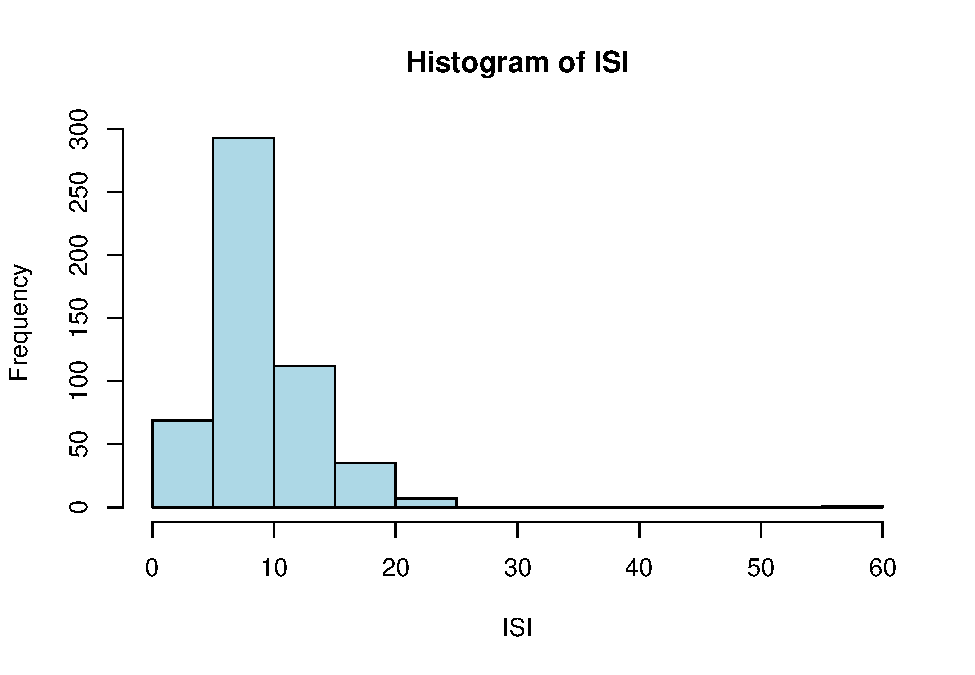
\includegraphics{forest_fires_files/figure-latex/unnamed-chunk-1-1.pdf}

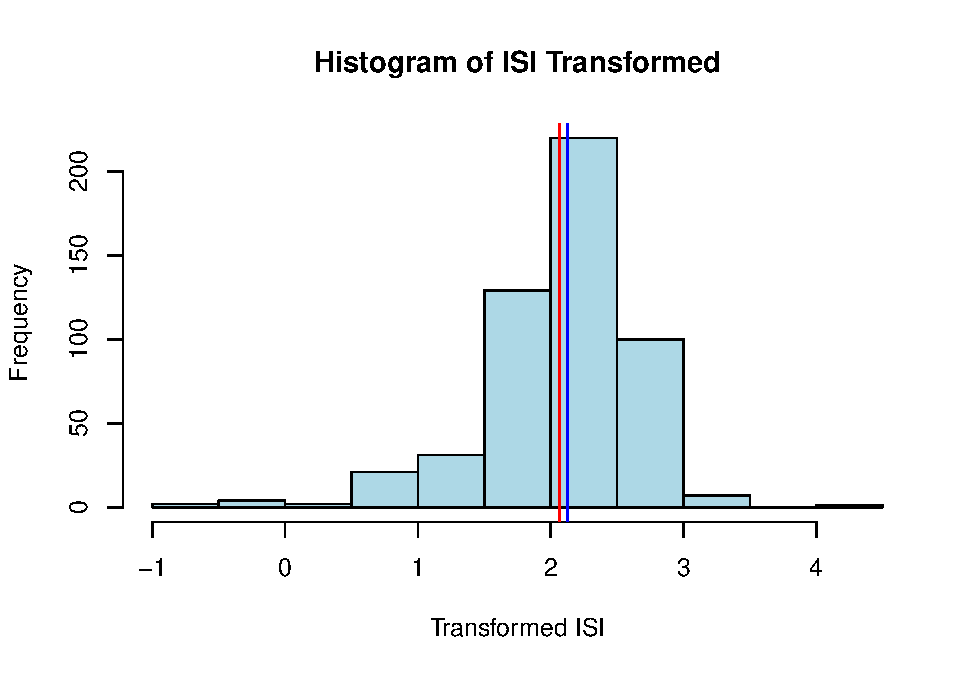
\includegraphics{forest_fires_files/figure-latex/transform-1.pdf}

The response variable of ISI was originally right-skewed. To prevent a
normality violation in the regressional model, the data is transformed
by taking the natural log of all ISI data. A QQ-normal plot is shown
below to illustrate that the residual data is normally distributed after
being transformed.

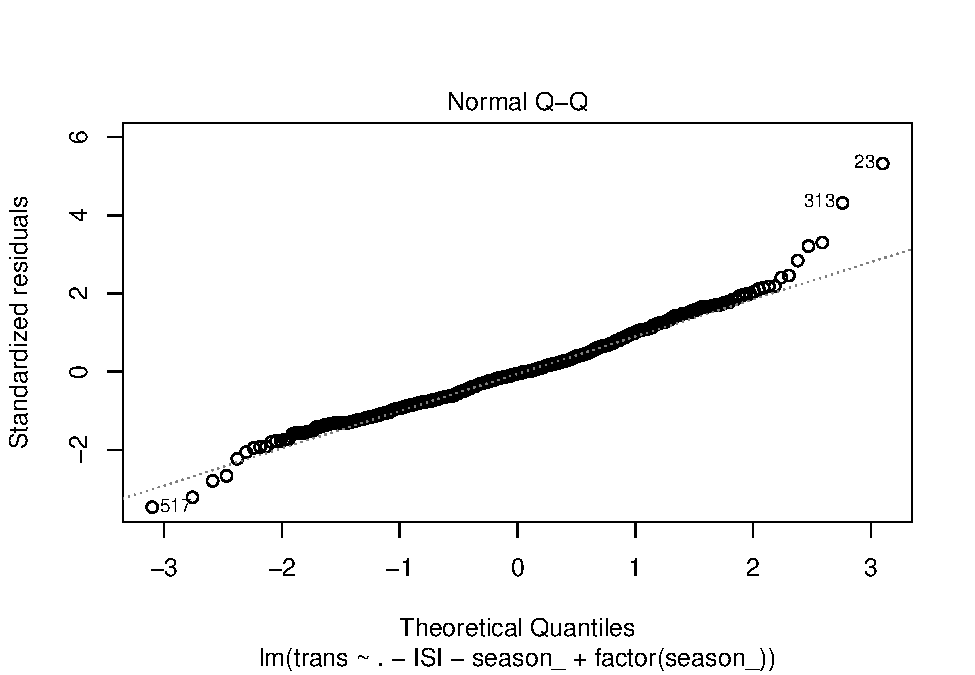
\includegraphics{forest_fires_files/figure-latex/unnamed-chunk-2-1.pdf}

\hypertarget{examining-multicolinearity}{%
\subsection{Examining
Multicolinearity}\label{examining-multicolinearity}}

Multicolinearity occurs when predictor variables are linearly correlated
with the other. This implies that a change in any one of the predictor
variables would entail a change in another highly correlated predictor
variable.

Before we proceed to fit our model it is important to perform two vital
checks. Firstly, there needs to be a reasonable correlation between the
predictor variables and the response variable. An absence of any linear
pattern does not warrant the use of a linear regression problem.

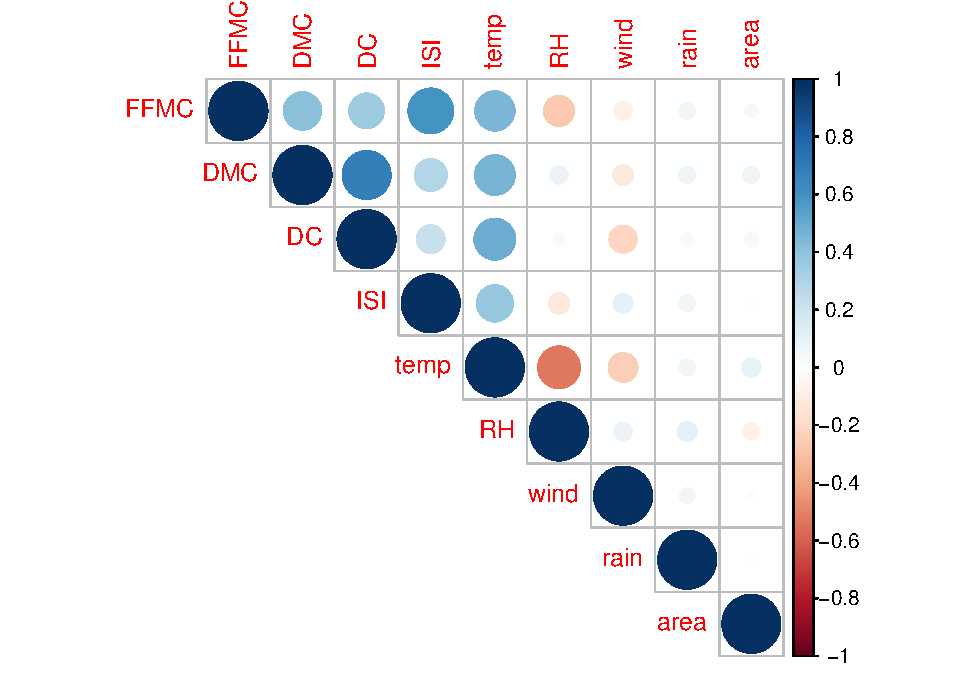
\includegraphics{forest_fires_files/figure-latex/unnamed-chunk-3-1.pdf}

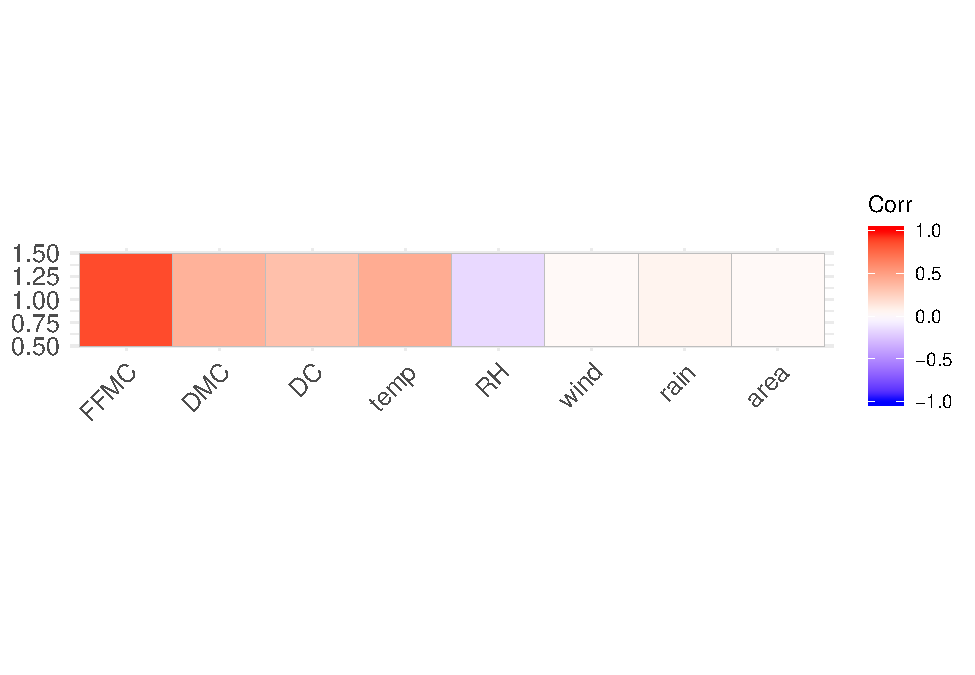
\includegraphics{forest_fires_files/figure-latex/analysis-1.pdf}

The visual analysis above shows us that there are several predictor
variables that possess a significant correlation strength with the
response variable (transformed ISI). Furthermore we also see that there
exists no significant multicolinearity between the predictor variables.
In general there always lies the possibility that variables within the
same domain will correlate with one another to an extent.

However to further confirm our claim, we will employ the use of the
Variance Inflation Factor analysis. This analysis allows us to support /
reject our claim using numerical proof. It is important to note that the
lower the VIF (lowest being 1), the less multicolinearity exists in our
dataset. A VIF of 5 represents industry standard acceptance rate for
multicolinearity as a small value indicates that the standard deviation
of the respective variable parameter will remain relatively stable when
other predictor variables are added into the regression equation.

\begin{Shaded}
\begin{Highlighting}[]
\CommentTok{#Calculate the Variance Inflation Factor for each of the predictor variables}
\NormalTok{model <-}\StringTok{ }\KeywordTok{lm}\NormalTok{(trans}\OperatorTok{~}\StringTok{ }\NormalTok{fire}\OperatorTok{$}\NormalTok{FFMC }\OperatorTok{+}\StringTok{ }\NormalTok{fire}\OperatorTok{$}\NormalTok{DMC }\OperatorTok{+}\StringTok{ }\NormalTok{fire}\OperatorTok{$}\NormalTok{DC }\OperatorTok{+}\StringTok{ }\NormalTok{fire}\OperatorTok{$}\NormalTok{temp }\OperatorTok{+}\StringTok{ }\NormalTok{fire}\OperatorTok{$}\NormalTok{RH }\OperatorTok{+}\StringTok{ }\NormalTok{fire}\OperatorTok{$}\NormalTok{wind }\OperatorTok{+}\StringTok{ }\NormalTok{fire}\OperatorTok{$}\NormalTok{rain }\OperatorTok{+}\StringTok{ }\NormalTok{fire}\OperatorTok{$}\NormalTok{area }\OperatorTok{+}\StringTok{ }\KeywordTok{factor}\NormalTok{(fire}\OperatorTok{$}\NormalTok{season_) , }\DataTypeTok{data =}\NormalTok{ fire)}
\CommentTok{#summary(model)}
\KeywordTok{vif}\NormalTok{(model)}
\end{Highlighting}
\end{Shaded}

\begin{verbatim}
##                           GVIF Df GVIF^(1/(2*Df))
## fire$FFMC             1.459696  1        1.208179
## fire$DMC              3.101415  1        1.761083
## fire$DC               9.060482  1        3.010063
## fire$temp             3.730699  1        1.931502
## fire$RH               2.198147  1        1.482615
## fire$wind             1.122068  1        1.059277
## fire$rain             1.058029  1        1.028605
## fire$area             1.023608  1        1.011735
## factor(fire$season_) 14.581963  3        1.563037
\end{verbatim}

Based on the data above, it further supports that there exists no
significant multicolinearity in the dataset. Most of the VIF values are
under 2.5 far below the industry threshold of 5.

\hypertarget{results}{%
\section{Results}\label{results}}

After analyzing the correlation of the predictor variables in the
dataset, the next steps comprise the following: 1. Feature Selection

\begin{enumerate}
\def\labelenumi{\arabic{enumi}.}
\setcounter{enumi}{1}
\item
  Model fitting using Training Data 
\item
  Analysis 
\end{enumerate}

\hypertarget{feature-selection}{%
\subsection{Feature Selection}\label{feature-selection}}

Using stepwise regression, we iterate through different possibilities of
a linear model and choose one with features yileding the best (lowest)
error metric.

The QQ-normal plot below illustrates the distribution of our data after
utilizing stepwise regression for feature selection.

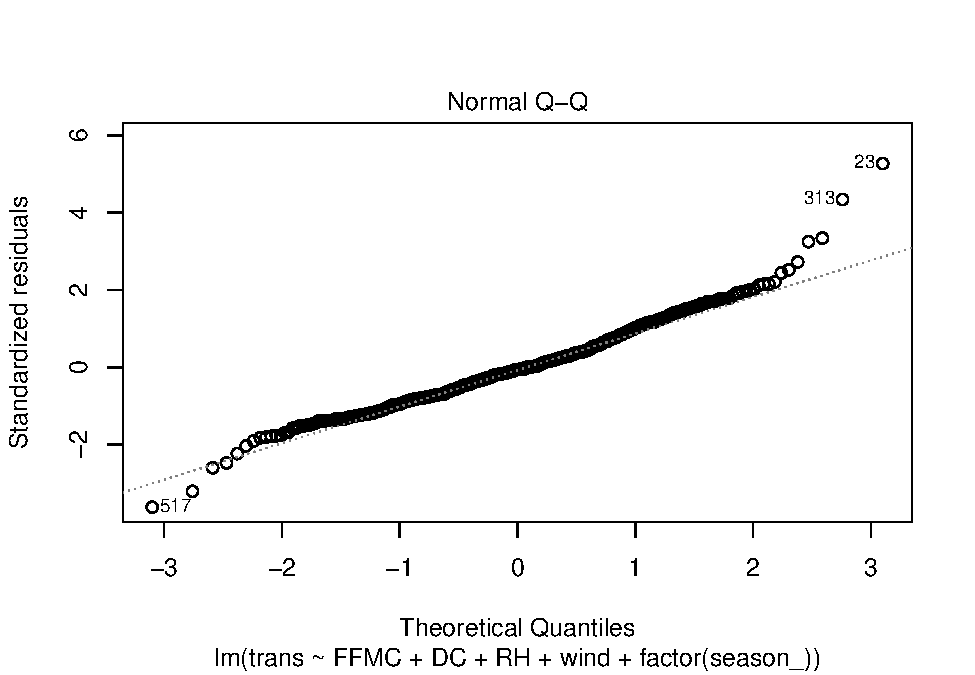
\includegraphics{forest_fires_files/figure-latex/unnamed-chunk-5-1.pdf}

\hypertarget{model-fitting}{%
\subsection{Model Fitting}\label{model-fitting}}

A portion of the data is separated to be utilized as a training set,
while the remaining portion will be utilized as a test set.This will
allow the accuracy of the model to be measured.

Next, the training data is fitted to the model with the selected
features. After removing features not selected from stepwise regression,
the model includes \texttt{factor(season\_)},\texttt{FFMC},
\texttt{temp}, \texttt{RH}, and \texttt{wind}

\hypertarget{analysis}{%
\subsection{Analysis}\label{analysis}}

The following conclusions are the results of our model:

\begin{itemize}
\item
  The overall P-value of the model is \textless{}2.2e-16. Being far
  below the indsutry standard of 5\% significance level, it can be
  concluded that at least one of the features is useful in predicting
  the response variable (ISI). Therefore the null hypothesis \(H_{0}\)
  is rejected.
\item
  The model yields an r-squared value of 0.76, indicating that it would
  likely be moderately useful in predicting the initial rate of spread
  of a fire.
\end{itemize}

\hypertarget{cooks-distance}{%
\subsection{Cook's Distance}\label{cooks-distance}}

After fitting the model, cook's distance is utilized to analyze if any
influential data points affect the regression line. If any exist, this
decreases the model's ability to generalize.

Based on the plot below, it can be confirmed that the training dataset
one outlier point (\textgreater{}1). This outlier point is also
influential in affecting the regression line of the model

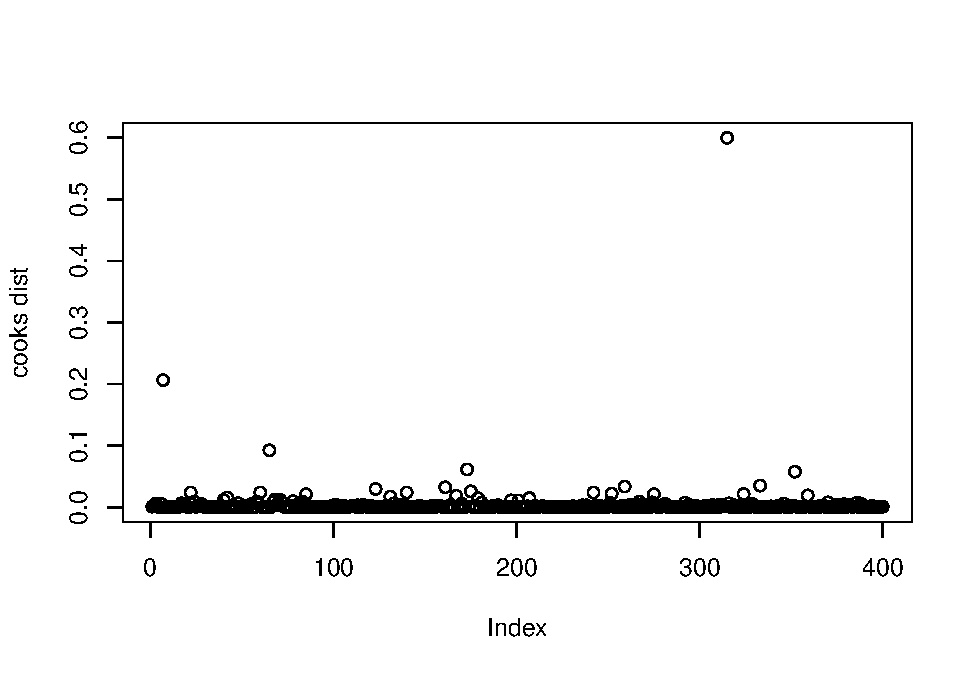
\includegraphics{forest_fires_files/figure-latex/unnamed-chunk-8-1.pdf}

\hypertarget{testing-the-model}{%
\subsection{Testing the Model}\label{testing-the-model}}

The model can be tested, and resulting mean squared error support our
conclusion that the model is moderately useful.

\hypertarget{conclusion}{%
\section{Conclusion}\label{conclusion}}

The conclusion goes here.

\hypertarget{acknowledgment}{%
\section{Acknowledgment}\label{acknowledgment}}

The authors would like to thank\ldots{} Dr.~Zarei

\hypertarget{references}{%
\section{References}\label{references}}

\newpage

\end{document}


